\chapter{系统实现}

\section{详细设计}

\subsection{用例设计}

一般用户在登录后可以上传视频并进行编辑、查询与管理编辑结果,并且可以查看开发者的相关信息。用户用例图如~\ref{fig:user_uml}所示。
\begin{figure}[ht]
    \centering
    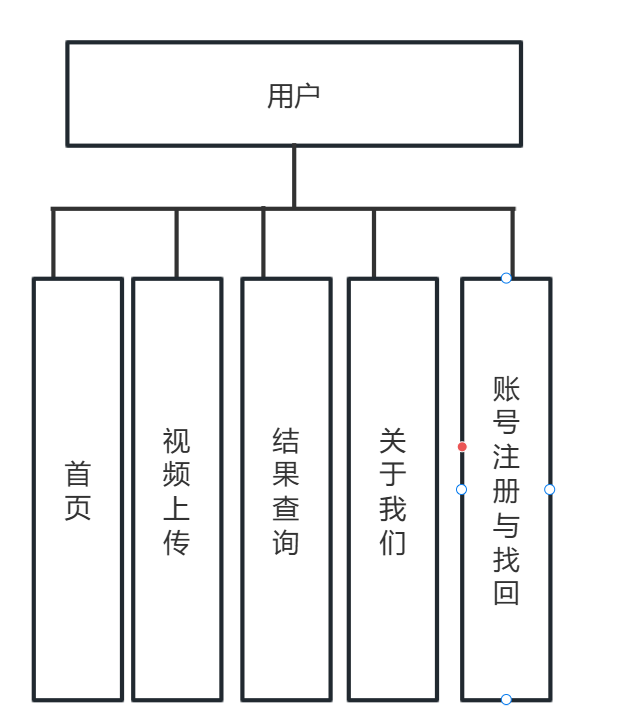
\includegraphics[width=0.3\textwidth]{source/img/user_uml.png}
    \bicaption{用户用例图}{User Use Case Diagram}
    \label{fig:user_uml}
\end{figure}
管理员用户除了一般用户所拥有的功能之外,还添加了数据统计与任务请求导出功能,以方便实验室研究者了解用户真实需求。管理员用户用例图如\ref{fig:admin_uml}所示。
\begin{figure}[ht]
    \centering
    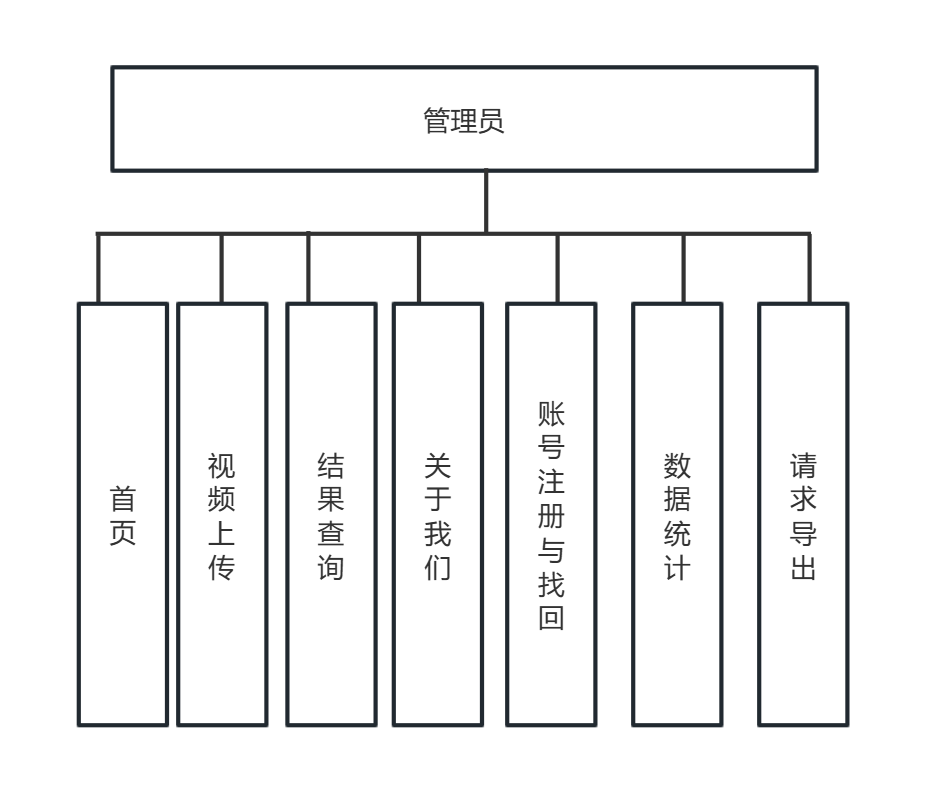
\includegraphics[width=0.4\textwidth]{source/img/admin_uml.png}
    \bicaption{管理员用例图}{Admin Use Case Diagram}
    \label{fig:admin_uml}
\end{figure}

\subsection{流程设计}

系统涉及到的工作流程主要包括登陆管理、任务上传与结果管理。

\subsubsection{登录管理}

由于用户的编辑结果通过邮箱来发送,我们可以将邮箱作为用户的唯一标识,在用户注册时将邮箱作为用户名,密码作为用户密码,通过邮箱和密码进行登录。
用户忘记密码时也可以通过邮箱进行密码重置。登录流程如\ref{fig:login_process}所示。
\begin{figure}[ht]
    \centering
    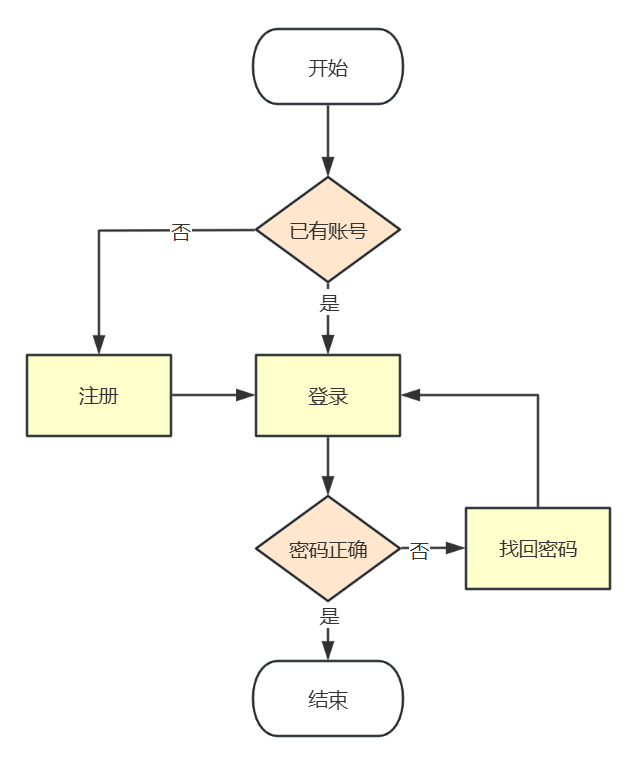
\includegraphics[width=0.4\textwidth]{source/img/login_process.png}
    \bicaption{登录流程图}{Login Process}
    \label{fig:login_process}
\end{figure}

\subsubsection{任务上传}

根据视频编辑算法的输入,需要用户提供视频、编辑提示类型与对应的提示内容,并提供邮箱以获取编辑结果。上传流程如\ref{fig:upload_process}所示。
\begin{figure}[ht]
    \centering
    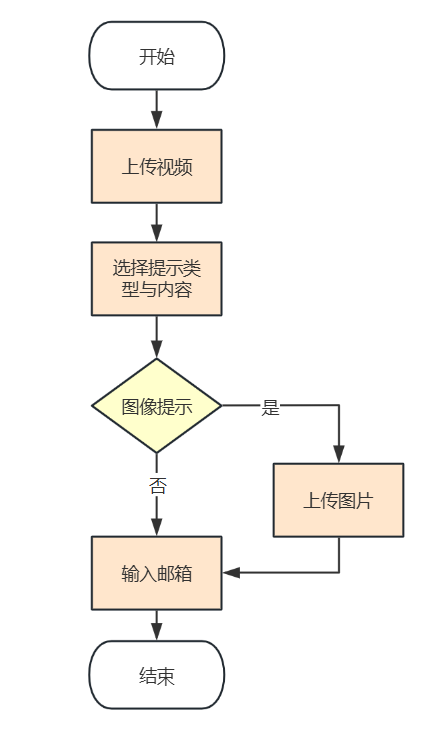
\includegraphics[width=0.3\textwidth]{source/img/edit_process.png}
    \bicaption{上传流程图}{Upload Process}
    \label{fig:upload_process}
\end{figure}

\subsubsection{结果管理}

用户在结果查询界面可以查看自己上传的任务进度与结果,系统也支持任务重命名与删除,同时在任务处理完成后会自动生成略缩图,方便用户预览结果。

\subsection{安全控制设计}

在系统构建的过程中,安全控制是一个至关重要的方面。为了防止未经授权的访问和操作,我们需要用户在登录状态下进行操作,这涉及到对用户信息与数据的
加密保护;我们也需要限制用户的操作行为,以防止用户的恶意操作;另外为了保证服务器的安全性,我们也需要系统部署过程中的安全措施。

\subsubsection{用户信息与数据加密}

我们将用户信息存储在数据库中,包括用户名、密码、邮箱等敏感信息。为了保证用户信息的安全性,我们对输入信息加密后存储。
我们使用密钥派生函数(Key Derivation Function, KDF)将用户提供的弱密码根据一些额外参数生成强密码,具体来说,
我们将用户的密码与给定的盐值(salt)连接起来,利用SHA256等加密函数经过多轮迭代得到最终的密码哈希值。由于哈希函数
具有单向性,我们无法通过哈希值反推原始密码,因此在验证用户密码时,我们只能重新计算哈希值并与存储的哈希值进行比较。

这种加密方式通过刻意使密钥派生的速度变慢,从而增加暴力破解的难度;同时由于不同密钥对应的盐值不同,确保了即使相同的密码
也会产生不同的哈希值,能够抵抗彩虹表攻击。

\subsubsection{用户行为限制}

为了防止用户恶意操作,如短时间大量上传文件、大量提交任务等,我们对用户行为做出一定的限制。具体包括:
\begin{itemize}
    \item 用户上传的文件在没有提交任务时被设置为一小时过期,未使用的文件达上限时拒绝用户的上传行为;
    \item 由于任务处理需要一定的时间,我们限制用户在处理的任务数量上限,超过限制则拒绝用户提交任务;
\end{itemize}
这些限制的具体实现通过MySQL数据库的触发器和在后台运行的定时任务完成。在插入数据时过期时间被设置为一小时后,当有任务使用到
对应文件时,UsedByProjectID字段外键引用任务ID;任务被删除时外键引用设置为NULL,触发器检测到后将时间设置为当前时间,文件过期。
后台的定时任务通过查询文件的过期时间字段来定时删除过期的文件。

\subsubsection{部署安全措施}

为了保证服务器的安全性,我们采取了以下措施:
\begin{itemize}
    \item 限制服务器中部署用户组的权限,避免系统文件遭到篡改;
    \item 文件传输使用HTTPS协议传输,通过SSL/TSL协议建立加密的传输通道
    \item 服务器部署在内网,限制外部访问,在网关上设置防火墙。
\end{itemize}